%%%%%%%%%%%%%%%%%%%%%%%%%%%%%%%%%%%%%%%%%%%%%%%%%%%%%%%
%
% AUTHOR: 李顺
%
% DESCRIBTION: 论文第一章部分
%
%
%%%%%%%%%%%%%%%%%%%%%%%%%%%%%%%%%%%%%%%%%%%%%%%%%%%%%%%

\chapter{绪论}
\label{chap:intro}
\section{选题的背景和意义}
无人机(UAV)技术在近年来得到了极其迅速的的发展。其中,尤其是固定翼无人机被广泛应用于现代战争之中。但是单架无人机往往限制较多,例如
:由于机载传感器尺寸、安装位置以及精度的限制,单架无人机往往不能快速全面的侦察某一广泛区域的战略目标;由于单架无人机机动性的限制,
单架无人机收到敌方打击而失效的概率大大增加。

而多架无人机进行编队控制从而进行协同作战可以使得无人机群体的战场存活率相较于单无人机系统更高。另外,通过图像拼接、协同滤波等技术
可以将编队侦查的无人机系统的信息融合为整个大环境的整体态势,因而
编队无人机对于战场的侦查效率也大大提高,对于单一传感器的精度的要求也相应降低。从而能
更好的完成领土保卫以及战场侦察任务。除此之外,无人机进行紧密编队还可
以实现长航程、长航时任务中无人机的空中加油等任务, 如图\ref{fig:c01-meaning}所示,从而进一步提高了无人机的作战能力以及适应复杂战场环境的能力。

固定翼无人机以紧密编队的形式飞行,如迁徙的鸟儿一样,可以减少整体的飞行阻力并且减少燃料消耗。整体编队产生的气动减阻效果将会
精心设计的、
具有良好的气动外形的飞行器相媲美。但是,按照相关文献显示,如果固定翼编队的控制精度无法达到要求精度的10\%,那么最优的减租效果
可能会被削减30\%。\cite{Zhang2017Aerodynamics}此外,固定翼编队避障也是热点问题之一:2019年,张佳龙等人对三架无人机的协同编队以及
其避障做了相关研究。\cite{Zzhangjialong2019Collision}

小型低成本固定翼无人机因其体积小巧、携带简单、部署容易以及成本低廉等优点,逐渐成为进行固定翼无人机编队实验的良好平台。\cite{Wangxiangke2019}通过现有的开源自动驾驶仪再结合机器人操作系统
配合商业级自动驾驶仪可以方便进行无人机编队的仿真以及实物试飞实验。
固定翼无人机编队飞行实现涉及队形规划、编队形成、队形保持与变换、协调通信甚至编队避障等领域。相较于四旋翼等空中机器人的编队,固定翼
因其动力学模型的复杂性,直接导致控制上的复杂性,进而使得固定翼自主编队的任务更加困难。另外因为控制硬件成本的低廉性,导致控制精度的下降,
使得编队控制将更加困难。本文旨在提出一种符合固定翼无人机动力学特性
的、基于当前较为成熟的开源无人机自动驾驶仪的固定翼紧密编队软件、硬件解决方案。
 \begin{figure}[H]
  \centering
  \subfigure[无人机编队加受油]{
  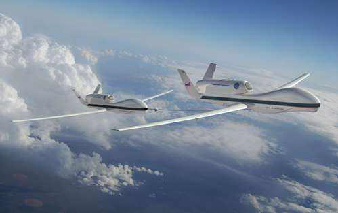
\includegraphics[width=0.45\textwidth, height=0.25\textwidth]{figures/c1/c01-meaning-1} 
}
  \subfigure[无人机编队巡航]{
  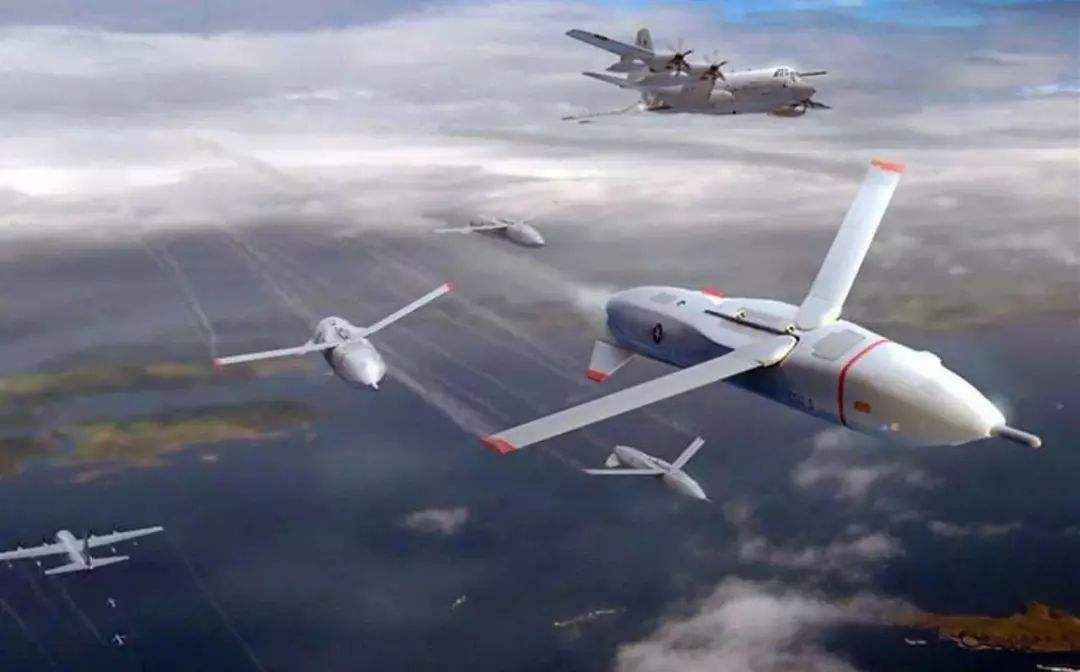
\includegraphics[width=0.45\textwidth, height=0.25\textwidth]{figures/c1/c01-meaning-2}
}
  \subfigure[无人机编队协同作战]{
  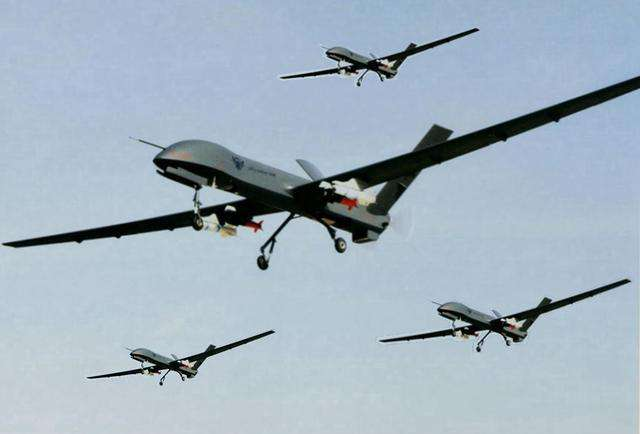
\includegraphics[width=0.45\textwidth, height=0.25\textwidth]{figures/c1/c01-meaning-3}
}
  \subfigure[无人机编队信息交互]{
  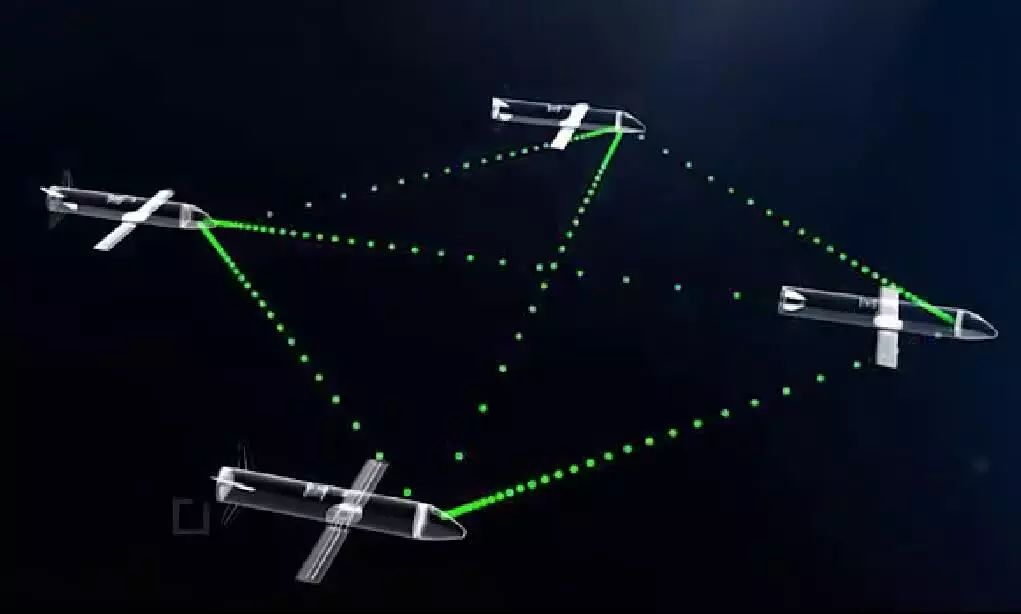
\includegraphics[width=0.45\textwidth, height=0.25\textwidth]{figures/c1/c01-meaning-4}
}
  \caption{无人机编队应用场景}
  \label{fig:c01-meaning}
  \end{figure}
\section{国内外研究现状及发展趋势}
\subsection{无人机自动驾驶仪发展}
自动驾驶仪作为无人机自主飞行的核心控制单元,是链接飞行任务以及无人机的软件、硬件桥梁。
成熟的无人机自驾仪应至少具备决策、航迹规划,状态感知和数据采集以及飞行控制等功能,从而实现无人机的全自主飞行,完成既定飞行任务。
任务的完成性。\cite{LiuLi2010}
现如今的开源无人机自动驾驶仪的结构多分为由导航模块、位置控制控制模块(外环)以及姿态控制模块(内环)等;其中,导航与位置模块的典型控制方
法有的就是L1控制器\cite{Park_2004}与TECS控制器\cite{Lambregts1983Vertical};导航模块产生期望位置,位置控制模块由期望位置产生
期望姿态角,姿态控制模块由期望姿态角产生最终的伺服系统的控制量。图\ref{fig-c1-autopilot}展示了一款典型的固定翼无人机自动驾驶仪逻辑。
\begin{figure}[H]
    \centering
    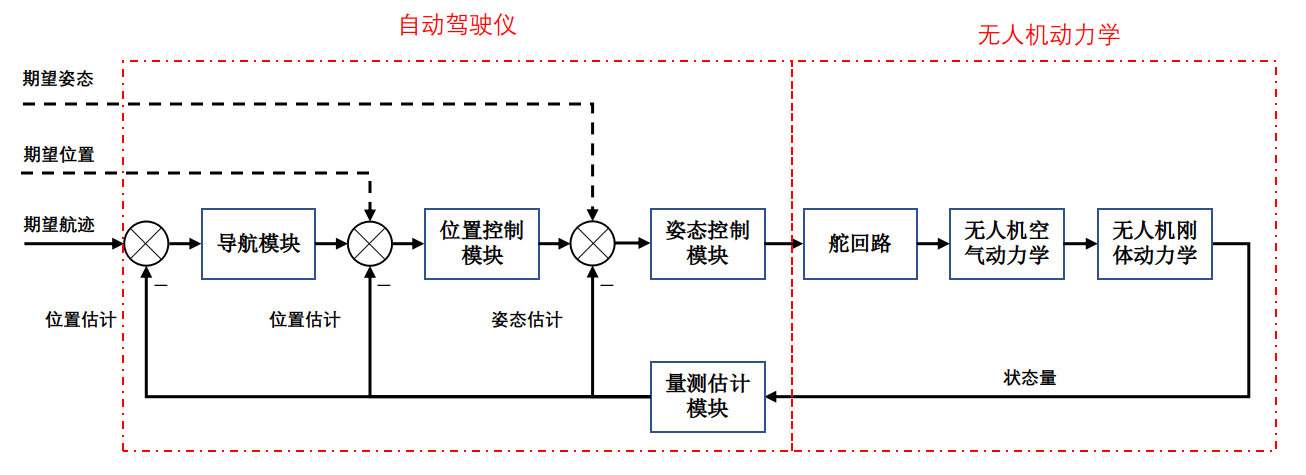
\includegraphics[width=0.85\textwidth]{figures/c1/autopilot_struct}
    \caption{典型无人机自动驾驶仪结构}\label{fig-c1-autopilot}
\end{figure}
\subsection{编队控制算法发展状况}
多无人机编队的最终目的是在空间之中形成固定的亦或是随时间变化的期望几何形状。为达成此目的,目前的编队控制领域已经提出多种解决方案:
\begin{enumerate}
    \item 领从方法(leader-follower method)\\
        此种方法本质而言是基于距离的编队方法(distance-based),因其原理简单,而得到广泛应用。
        领从方法的大致思路为:领航无人机按照预先设定的轨迹飞行,跟随无人机以期望编队位置的距离误差,与领航无人机速度误差作为误差
        输入,设计相应的控制器,最终使得误差消除,达到编队目的。2007年,西北工业大学的朱战霞、郑莉莉设计了基于PI控制器的编队控制器,
        提出了编队的混合误差定义。\cite{ZhuZhanXia2007}
        2008年,王莉等人针对多无人车系统,利用基本的领从方法进行编队算法设计。\cite{WangLi2008}
        2012年,Turpin等人提出了改进的leader-follower 编队算法,使得编队中
        任意一架无人机通过与自己相邻节点(无人机)之间进行通讯来获得领机的状态信息,从而减轻了领机节点的通讯压力。
        \cite{Turpin2012Trajectory}同组的Saska等利用机载感知设备实现了无GPS定位条件下的的密集飞行任务。\cite{Saska2017System}魏扬等人在2016年
        设计出一款基于PID控制器的输出控制量为期望加速度以及偏航角的编队控制器,并对其做了稳定性的数学证明。\cite{WeiYang2016}
    \item 基于行为方法\\
        此种方法的大致思路是将无人机的完整任务划分为几种多种行为,例如:跟随、队形保持、队形变换以及避障等。对于不同行为的加权作为最终无人机的
        “控制行为”。1998年,Arkin等人为解决多智能体编队控制问题而提出了一种基于行为的编队控制方法。\cite{Balch1998Behavior} 2009年,
        R.K.Sharma等人将基于行为法进行改进,以解决编队控制中的避障问题。\cite{Sharma2009Collision} 近年来,也有学者对某些生物(如鸟群)行为进行分析归纳
        ,并通过类似行为分析的方法引入编队控制中。
        2003年,美国 Jadbabaie 等人为了对基于行为法进行深入的研究,提出了最近邻近协调的思想。\cite{Jadbabaie2003Coordination}Kim等在2009年设计出一种基于反馈线
        性化方法设计的分布式控制器。\cite{Kim2009}学宋运忠等人在2012 年,利用线性手段解非线性的物理模型方程,解决了多智能体系统队形控
        制问题,改进了智能体基于行为的编队控制方法。\cite{SongYunZhong2012}近年来仿生学也被应用到编队控制的研究之中来:2015年,段海滨团队建立了鸽群行为机制模型,提出了鸽群
        行为编队控制算法。\cite{DuanHaiBin2015}
        Shin等在同一年将协同控制引入基于行为的编队控制之中,提出了分布式编队控制策略,使得网络中的节点处理邻居的状态信息,提高了整体控制的鲁棒性。\cite{Jongho2015}
    \item 虚拟结构法\\
        虚拟结构法的中心思想是将编队的多个智能体(无人机)节点所组成的几何形状看作虚拟刚体,设计虚拟刚体中有一个虚拟领机或者位置为几何中心,刚体中的所有无人机
        均以此中线点为参考进行编队。\cite{Lewis1997High}
        此种算法最初应用于集中式算法设计中,但随着相关研究的深入,也有研究者将分布式算法以及虚拟结构法进行结合:
        任伟等结合一致性算法与虚拟结构法,对带干扰的便对运动问题进行反馈控制求解\cite{Ren2004Formation};在其另一篇论文中,任伟结合一致性算法与虚拟结
        构法,对集中式的虚拟结构法进行分布式求解,提出了分布式算法解决编队问题。\cite{Ren2004Decentralized}
\end{enumerate}

最近几年新型的控制器逐渐被应用到编队控制器的设计之中:2011年,西北工业大学肖亚辉等人针对无人机的三维编队设计了一种具有良好鲁棒性的模糊PID控制器,进而控制无人机的三维编队。\cite{XiaoYaHui2011}
2018年,南京航空航天大学的许玥将自适应容错控制器引入到编队控制器的设计之中来。\cite{XuYue} 2019年,赵菁祥等人设计了编队控制的
滑膜控制器。2020年,北京理工大学的强久佳设计了参数优化自抗扰固定翼无人机编队控制器。\cite{MengXiuyun2020}近年来,还有的学者考虑到无人机编队问题中的时变问题,
并作出了先关的研究,例如:何吕龙等人利用图论的相关知识研究通信拓扑等相关问题\cite{Helvlong2020};类似的还有周绍磊\cite{Zhoushaolei2020}、张西勇\cite{Zhangxiyong2019}等人的研究;
董朝阳\cite{Dongzhaoyang2020}、季蕾\cite{Jilei2019}、徐振\cite{Xuzhen2019}等人则研究了编队结构中的时变问题。

现如今已经存在的大部分编队控制算法均为考虑飞机的质点运动学以及质点动力学条件下提
出的导航方法,最终产生的飞行器的控制量为无人机航迹坐标系下的加速度期望值以及无人机的航向角的期望角速度。例如:朱战霞、魏扬等人所设计的编队控制器
按照飞机的控制方式,需要将航迹坐标系下的
期望控制量转到机体系之下,但是飞机自动驾驶仪并不能接受加速度控制量,尤其是飞机机体$O_bx_b$轴方向,无人机推力、阻力以及重力沿机体方
向的推力并非是代数关系,不能直接由期望加速度得到期望推力;无人机姿态驾驶仪常使用协调转弯模型作为内环角度环的控制基础,不能直接响应
所给出的偏航角速度的期望值。2019年吉林大学的张天慧基于上述介绍的领从方法,利用地面站与自动驾驶仪系统设计固定翼编队控制器,\cite{Zhangtianhui2019}但是
其方法规划与运算由地面站完成,延时以及不确定性相较机载计算平台增加。总结而言即:
当前的大部分编队控制律不能很好的与自动驾驶仪内环相结合结合。
但是现如今的低成本无人机所使用的传感器硬件精度比较低,均为消费级别,如果不考虑传感器的精度问题而设计控制方案,很可能导致整体编队的控制精度下降。
另外由于低成
本无人机的惯性原件的精度问题导致无人机不能使用测量的加速度信息作为反馈,两种原因导致以加速度为最终控制量对于低成本无人机编队的方法控制精度不足。
\section{本文的内容安排}
本文中的编队控制器设计主要基于领从方法,从无人机编队的距离、速度大小以及速度方向误差出发,设计符合现有无人机内环姿态驾驶仪输入的
编队控制器。
本文之后的部分将如下组织:第二章首先介绍编队控制设计的假设以及所用到的坐标系,最终建立建立无人机编队的动力学模型;第三章介绍自动驾驶仪的控制逻辑:包括导航、位置控制以及姿态控制等模块的实现。第四章首先
完成对于编队误差的定义,将所定义的编队误差作为输入、无人机内环姿态驾驶仪期望姿态作为输出,设计编队控制器数学形式;第五章介绍
无人机编队整体控制逻辑、动力学仿真环境以及硬件选型 ;第六章控制器仿真以及实际飞行实验结果分析;最后为结论。
